\minitoc% Creating an actual minitoc
Programming robots for general purpose applications is extremely challenging due to the great diversity of end-user tasks.
Not only is it generally left up to robotics experts, but end-user programming solutions are often limited to teaching robots predefined actions for specific tasks that cannot be reused.
This thesis argues for letting end-users teach robots primitive or \textit{atomic} actions from scratch that can be reused with task planners for previously unseen problems.
In this way, we delegate the logical reasoning process of finding a solution to task planners and facilitate the robot programming process, while maintaining the generalisability of taught actions.

This part of the thesis contains our contributions.
In this chapter we present iRoPro, an interactive Robot Programming framework and discuss its theoretic components.
The framework combines Programming by Demonstration and Automated Planning techniques for goal-oriented robot programming by end-users.
We end this chapter by discussing the research methodology used in this thesis which resulted in the contributions presented in the remaining chapters (\sect{sec:methodology}).
%We conduct qualitative user experiments to analyse the user's understanding when first presented to basic concepts in Automated Planning and Programming by Demonstration (\chapt{chap:Pre-Experiments}).
%We then focus on goal-oriented robot programming, where users simultaneously teach robots actions and goals by demonstration (\chapt{chap:OrganisingTasks}).
%Finally, we present the iRoPro implementation as a working end-to-end system that allows users to teach robots low- and high-level actions that can be reused with task planners to solve previously unseen problems (\chapt{chap:Implementation}).
%We evaluate the system implemented on a Baxter robot and present experimental findings from a user study. %(\chapt{chap:Evaluation}).
%We conclude this thesis by discussing limitations and potential future work (\chapt{chap:Conclusion}).

\newpage
\section{iRoPro - interactive Robot Programming}
iRoPro, an interactive Robot Programming, is a framework that allows end-users to teach robots primitive actions from scratch that can be reused with task planners.
%a goal-oriented behaviour and 
The framework consists of the following three components (\fig{fig:framework}): 
\begin{enumerate}
	\item[A.]{Programming by Demonstration: The user \textit{teaches} the robot primitive actions by demonstration. The robot creates an action model that the user can refine and validate.}
	\item[B.]{Automated Planning: The user defines a new planning problem with a goal to achieve. The robot which \textit{reuses} the taught actions with a planner to generate a solutions for new problems.}
	\item[C.]{Retro-active Loop: The user observes the robot execution and \textit{refines} taught actions via the graphical interface.}
\end{enumerate}
%Similar to other approaches (\cite{perzylo2016intuitive}), 
The user is provided with a graphical user interface (GUI) that abstracts from the underlying modeling language used for automated planning.
For each step, the user interacts with the GUI to navigate between the components to teach new actions by demonstration, modify inferred action conditions, define new planning problems for the robot to solve and execute generated plans.
In the following sections, we discuss each component in more detail. 
%We refer the reader to a video of the framework: \texttt{https://youtu.be/DTm2YjiSNQM}
%Using this knowledge base, the user can define a planning problem, for which the robot will generate a plan. 

\begin{figure}[!h]
	\centering
	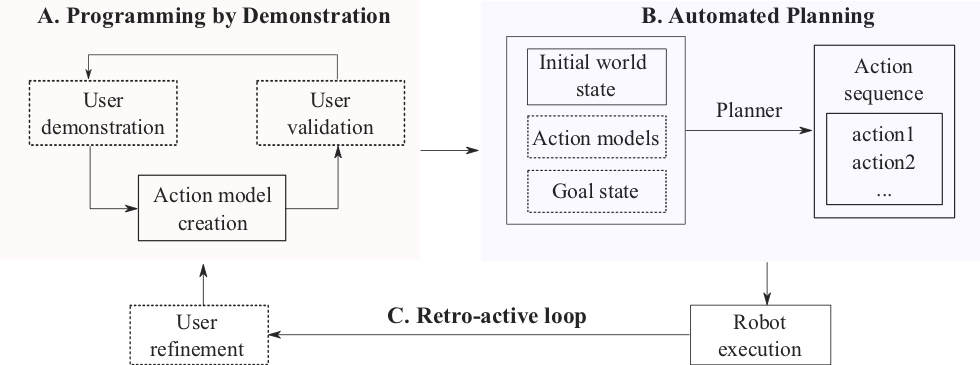
\includegraphics[width=\linewidth]{figures/framework.png}
	\caption{An overview of the iRoPro (interactive Robot Programming) framework: A. the user teaches primitive actions by demonstration B. the robot reuses these with a task planner to generate an action sequence to achieve a goal.
	C. After observing the robot execution, the user can refine the taught action models (dotted lines indicate user actions, solid lines indicate robot actions).}
	\label{fig:framework}
\end{figure}

\subsection{Programming by Demonstration: teaching actions}
%Our approach aims at providing end-users with an intuitive way of 
Teaching robots atomic actions consists of learning both \textit{how} and \textit{when} an action should be applied, \ie the low-level (\sect{ssec:lowlevel}) and high-level representations (\sect{ssec:highlevel}) respectively.
We consider an action that consists of both low- and high-level representations an \textit{action model}.
To teach action models, Programming by demonstration (PbD) (\sect{sssec:PbD}) can be used as an intuitive end-users programming approach.
%gripper states (open/close) and end-effector poses relative to perceived objects or to the robot's coordinate frame.
Low-level actions can be learned from multiple demonstrations (\cite{niekum2012learning}) or a single demonstration, where poses are assigned heuristically and corrected by the user if needed (\cite{alexandrova2014robot}).
Dynamic Movement Primitives (\cite{pastor2009learning}) or mixture models (\cite{calinon2007incremental}) learn actions from entire motion trajectories but generally require multiple demonstrations (\cite{abdo2013learning}).
\cite{ahmadzadeh2013visuospatial} generates trajectories by extracting three key points that represent the \textit{rest, pick} and \textit{place} actions of an object.
In keyframe-based PbD (\cite{akgun2012keyframe,alexandrova2014robot}), actions are represented as a sparse sequence of keyframes that can be connected to perform a skill.

The user can teach multiple low-level actions and discriminate between them by associating different high-level conditions that specify \textit{when} the robot should use the action. % (\eg actions using claw or suction grippers).
In iRoPro, high-level actions are represented similar to planning operators in automated planning (\sect{subsec:Classical planning problem}), where an action is a tuple $o = (\text{name}(o), \text{precond}(o),$ $\text{effect}(o))$ with preconditions and effects.
% are represented in terms of predicates, \eg object properties, that describe the current state of the world.
State-of-the-art perception systems (\eg SIFT (\cite{ahmadzadeh2015learning})) or a database of object features (\cite{mason2011robot})) are used to automatically recognise object properties such as type, position, or spatial relation relative to other objects.
When the user demonstrates an action, such as pick-and-place of a cube, %\texttt{(move cube A B)}.
it results in a change in the world state, \eg the cube's position changes from A to B.
The robot observes the world state before and after the action demonstration, and infers relevant predicates for preconditions and effects to build an action model. %, expressed in a symbolic planning language.% (Fig. \ref{fig:action} bottom).
Predicates can be inferred from observing what changed or what stayed the same in the state of the world.
Feature-based algorithms, such as k-means clustering, can be used to learn high-level action conditions from multiple demonstrations (\cite{mollard2015robot,abdo2013learning}).
Existing PbD approaches try to teach the robot from a small number of demonstrations, but require at least five contextually different ones (\cite{orendt2016robot,abdo2013learning}).
%To learn object manipulation tasks, the robot perceives the initial world state before %(\textit{precondition}) and after the action demonstration and infers the high-level conditions (\cite{ahmadzadeh2015learning}).
%(\textit{effects}). 
In iRoPro, we propose an interactive programming approach, where the user can directly modify learned action models via the graphical interface.
Relying on the user's logical reasoning and understanding of what they want to teach the robot, we allow them to directly program and correct action models.
Thus, the robot can learn a new action from a single demonstration with the user acting as the expert to correct inferred conditions.
The user validates the learned action model or provides additional demonstrations to refine the low- or high-level representations.
The user repeats this process and creates an action model for each unique primitive action.
%The robot learns from multiple demonstrations to generalise trajectories and high-level conditions.
%In the framework, we assume that the learned action trajectory is independent of the trajectory performed by the teacher.

%Note that we do not address the perception problem in this paper. 
%In our experiments, we implemented a simple python algorithm with integrated functionalities of the Robot Operating System (ROS) (\cite{quigley2009ros}), to detect and move objects, based on their colour.

%Table \ref{tab:action-model} shows the states of the demonstrated action and the generalised action model. 
%The generalised operator is automatically translated into a symbolic representation, allowing the creation of a planning domain, without the need for any programming knowledge.


\subsection{Automated Planning: reusing actions}\label{sec:AP}
In the PbD step, the robot learned action models that include the high-level representation that is used in Automated Planning. 
The Automated Planning step consists of creating an planning problem, defining a task goal and generating a solution to the solve the problem.
Task planners are used to generate solutions to solve complex problems (\chapt{chap:Sota-AP}).
Various planners have been used for robotic task planning, such as the STRIPS planner (\cite{she2014teaching}), Metric-FF (\cite{cubek2015high}), fast downward planner (\cite{abdo2013learning}). 
Given a description of a planning \textit{domain}, \ie object types, predicates, and actions, we can define a planning \textit{problem} with an initial state and a desired goal state to achieve. 
The planner generates an optimal action sequence, or \textit{plan}, which guarantees the transition from initial state to the goal state. 
%Automated planners try to model the robot's strategies, when operating in diverse environments \cite{ghallab2004automated}.
%ught actions are reused with existing task planners by translating them into PDDL (\citet{mcdermott1998pddl}). 

Depending on the robot architecture and perception system, iRoPro integrates a partial PDDL domain including a set of object types and their predicates that the robot can recognise.
The previously created action models complete the partial PDDL domain.
% and manually adding custom types and predicates via the user interface.
Using the graphical interface, the user can create a new planning problem by detecting the initial world state and defining a goal to achieve.
The predicates for the initial world state are automatically inferred by the robot as in the PbD phase.
The user can modify and correct them via the interface. 
Then they enter predicates that describe a goal for the robot to achieve.
The task planner generates a plan, consisting of an ordered action sequence for the robot to execute. 
The user can verify the generated plan and have the robot execute it in real life.
If no plan is generated or if the plan seems incorrect, the user can modify the taught actions, as well as the initial and goal states and relaunch the planner.

\subsection{Retro-active Loop: refining actions}
The retro-active loop allows the user to revisit and correct created action models.
%Generating a plan under different initial states allows the user to test the created action models.
It is likely that the initially generated plan does not produce the desired outcome, especially if the context of the planning problem is different to that of the initial demonstration (\eg different object types or positions).
To minimise the user's programming process and the number of demonstrations required, taught actions can be generalised and reused, especially if the low-level action is similar.
Instead of creating new action models for each new problem, the user can revisit and modify existing ones so that they are reused by the planner.
Thus, the application to a new context is an important step to test the generalisability of action models.
There are several possible causes for suboptimal, incorrect or non-existent solutions generated by the planner:
\begin{itemize}
	\item \textbf{Object types:} they dictate what objects an action can be applied to. If they do not match those of the observed world state in the current planning problem, the action is not considered by the planner (\eg pick-and-place was only defined for cube objects but not other types).
	\item \textbf{Preconditions:} they define when an action can be applied. If they do not match the observed world state, the planner could make wrong assumptions about the usage of taught actions (\eg pick-and-place of an object that is not clear).
	\item \textbf{Effects:} they define how the world state is updated after the action execution and help the robot to keep track of changes. If they are not defined correctly, there can be a mismatch of the robot's perceived world state and the actual world state (\eg a position is still considered free when it is occupied).
	\item \textbf{Initial world states:} they describe the existing world state of objects to the robot. If the initial world state is incorrect the planner may consider certain actions as invalid due to their defined preconditions.
	\item \textbf{Goal:} this defines the minimal set of predicates that need to be achieved and should not include consequent states or intermediate steps to achieve the goal. Contradicting goal states automatically lead to non-existing plans (\eg `object is on A' and `A is clear' are stated as goal states).
\end{itemize}

Knowledge engineering tools (\sect{subsec:Knowledge Engineering}) can facilitate this process of modifying action models.
They often provide useful functionalities for dynamic testing, model checking and visualisation (\cite{simpson2007planning}), but most tools require expertise in automated planning or Software Engineering.
%where the quality of the models generated does not depend on the user's expertise.
In this thesis we argue that the proposed robot programming process does not require this expertise and can be learned easily by users with different educational backgrounds.


\section{Methodology}\label{sec:methodology}
The contributions in this thesis were constructed using both quantitative and qualitative research methodologies.
Our general approach follows the design wheel of the concept design process (\cite{designwheel}) consisting of successive cycles of `Explore', `Create', `Evaluate' and `Manage' phases (\fig{fig:designwheel}).
Our contributions represent the following stages:
\begin{enumerate}
	\item {\textbf{Pre-Experiments: }We start by conducting initial qualitative user experiments to investigate how end-users adopt basic concepts in Automated Planning and Programming by Demonstration.
	We are particularly interested in the difficulties they encounter when learning and applying automated planning concepts as they can be considered in the iRoPro system implementation.
	For this we create an initial prototype used for simulating iRoPro with the Wizard-of-Oz technique (\chapt{chap:Pre-Experiments}).
	}
	\item {\textbf{Goal-oriented Programming: }We then explore goal-oriented end-user programming approaches by allowing users to simultaneously teach the robot actions and goals by demonstration.
	For this we implement a system that includes learning new actions by demonstration and a graphical interface. We evaluate the system in an online user study on Amazon Mechanical Turk (\chapt{chap:OrganisingTasks}).}
	\item {\textbf{End-to-end System Implementation:} Taking the existing work as a basis, we implement iRoPro on a Baxter robot to allow simultaneous teaching of low- and high-level actions by demonstration.
	The end-to-end system includes a graphical interface that users interact with directly to teach, reuse and refine new action models (\chapt{chap:Implementation}).}
	\item {\textbf{Post-Experiments: } We conclude this thesis work by conducting further user experiments using the implemented system.
		We compare user groups with different educational backgrounds and investigate their performance on how they learn and use the system for programming the robot.
		We close the concept design process by comparing the latest user study with our initial experiments conducted at the start of this thesis work (\sect{sec:quanteval}).}
\end{enumerate}


\begin{figure}[h]
	\centering
	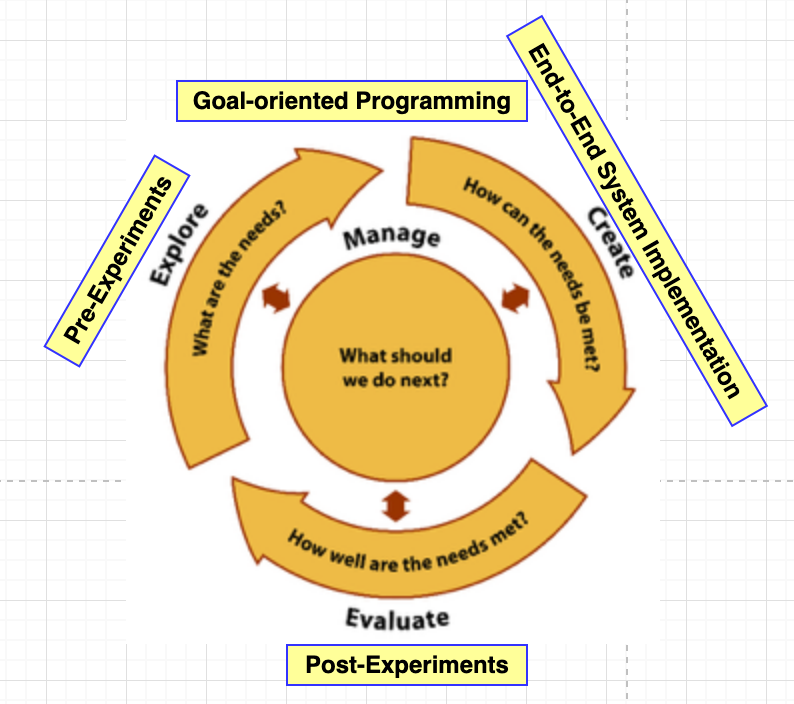
\includegraphics[width=0.83\linewidth]{figures/designwheel}
	\caption{The thesis contributions align with the design wheel consisting of successive cycles of `Explore', `Create', `Evaluate' and `Manage' phases  (\cite{designwheel}).}
	\label{fig:designwheel}
\end{figure}
